% Requires: \usepackage{tikz,pdflscape,float}
% \usetikzlibrary{arrows.meta,positioning,calc,shapes.geometric}
% Compile with pdflatex (or xelatex/lualatex for direct UTF-8 accents).
\documentclass{article}
\usepackage[margin=1cm]{geometry}
\usepackage[utf8]{inputenc}
\usepackage[T1]{fontenc}
\usepackage{pdflscape}
\usepackage{float}
\usepackage{tikz}
\usetikzlibrary{arrows.meta,positioning,calc,shapes.geometric}

\definecolor{l1blue}{HTML}{2F5FA8}
\definecolor{l2violet}{HTML}{6A3DA8}
\definecolor{l3green}{HTML}{2E8B57}

\tikzset{
  io/.style={rectangle, rounded corners=3pt, draw=black, very thick,
    fill=black!78, text=white, font=\bfseries\footnotesize,
    align=center, text width=6cm, inner sep=6pt},
  layer1/.style={rectangle, rounded corners=3pt, draw=l1blue, thick,
    fill=l1blue!10, text=black, font=\footnotesize, align=left,
    text width=6cm, inner sep=6pt},
  layer2/.style={rectangle, rounded corners=3pt, draw=l2violet, thick,
    fill=l2violet!10, text=black, font=\footnotesize, align=left,
    text width=6.6cm, inner sep=6pt},
  layer3/.style={rectangle, rounded corners=3pt, draw=l3green, thick,
    fill=l3green!10, text=black, font=\footnotesize, align=left,
    text width=7cm, inner sep=6pt},
  decision/.style={diamond, draw=black, thick, fill=yellow!12, aspect=2.4,
    font=\bfseries\footnotesize, align=center, text width=2.6cm, inner sep=2pt},
  accept/.style={rectangle, rounded corners=3pt, draw=teal!65!black, very thick,
    fill=teal!12, font=\bfseries\footnotesize, align=center,
    text width=3.6cm, inner sep=6pt},
  reject/.style={rectangle, rounded corners=3pt, draw=red!65!black, very thick,
    fill=red!8, font=\bfseries\footnotesize, align=center,
    text width=3.2cm, inner sep=6pt},
  arr1/.style={-{Latex[length=2.2mm]}, thick, l1blue},
  arr2/.style={-{Latex[length=2.2mm]}, thick, l2violet},
  arr3/.style={-{Latex[length=2.2mm]}, thick, l3green},
  arrdark/.style={-{Latex[length=2.2mm]}, thick, black},
  arracc/.style={-{Latex[length=2.2mm]}, thick, teal!65!black},
  arrrej/.style={-{Latex[length=2.2mm]}, thick, dashed, red!65!black},
}

\begin{document}
\begin{landscape}
\begin{figure}[H]
\centering
\small
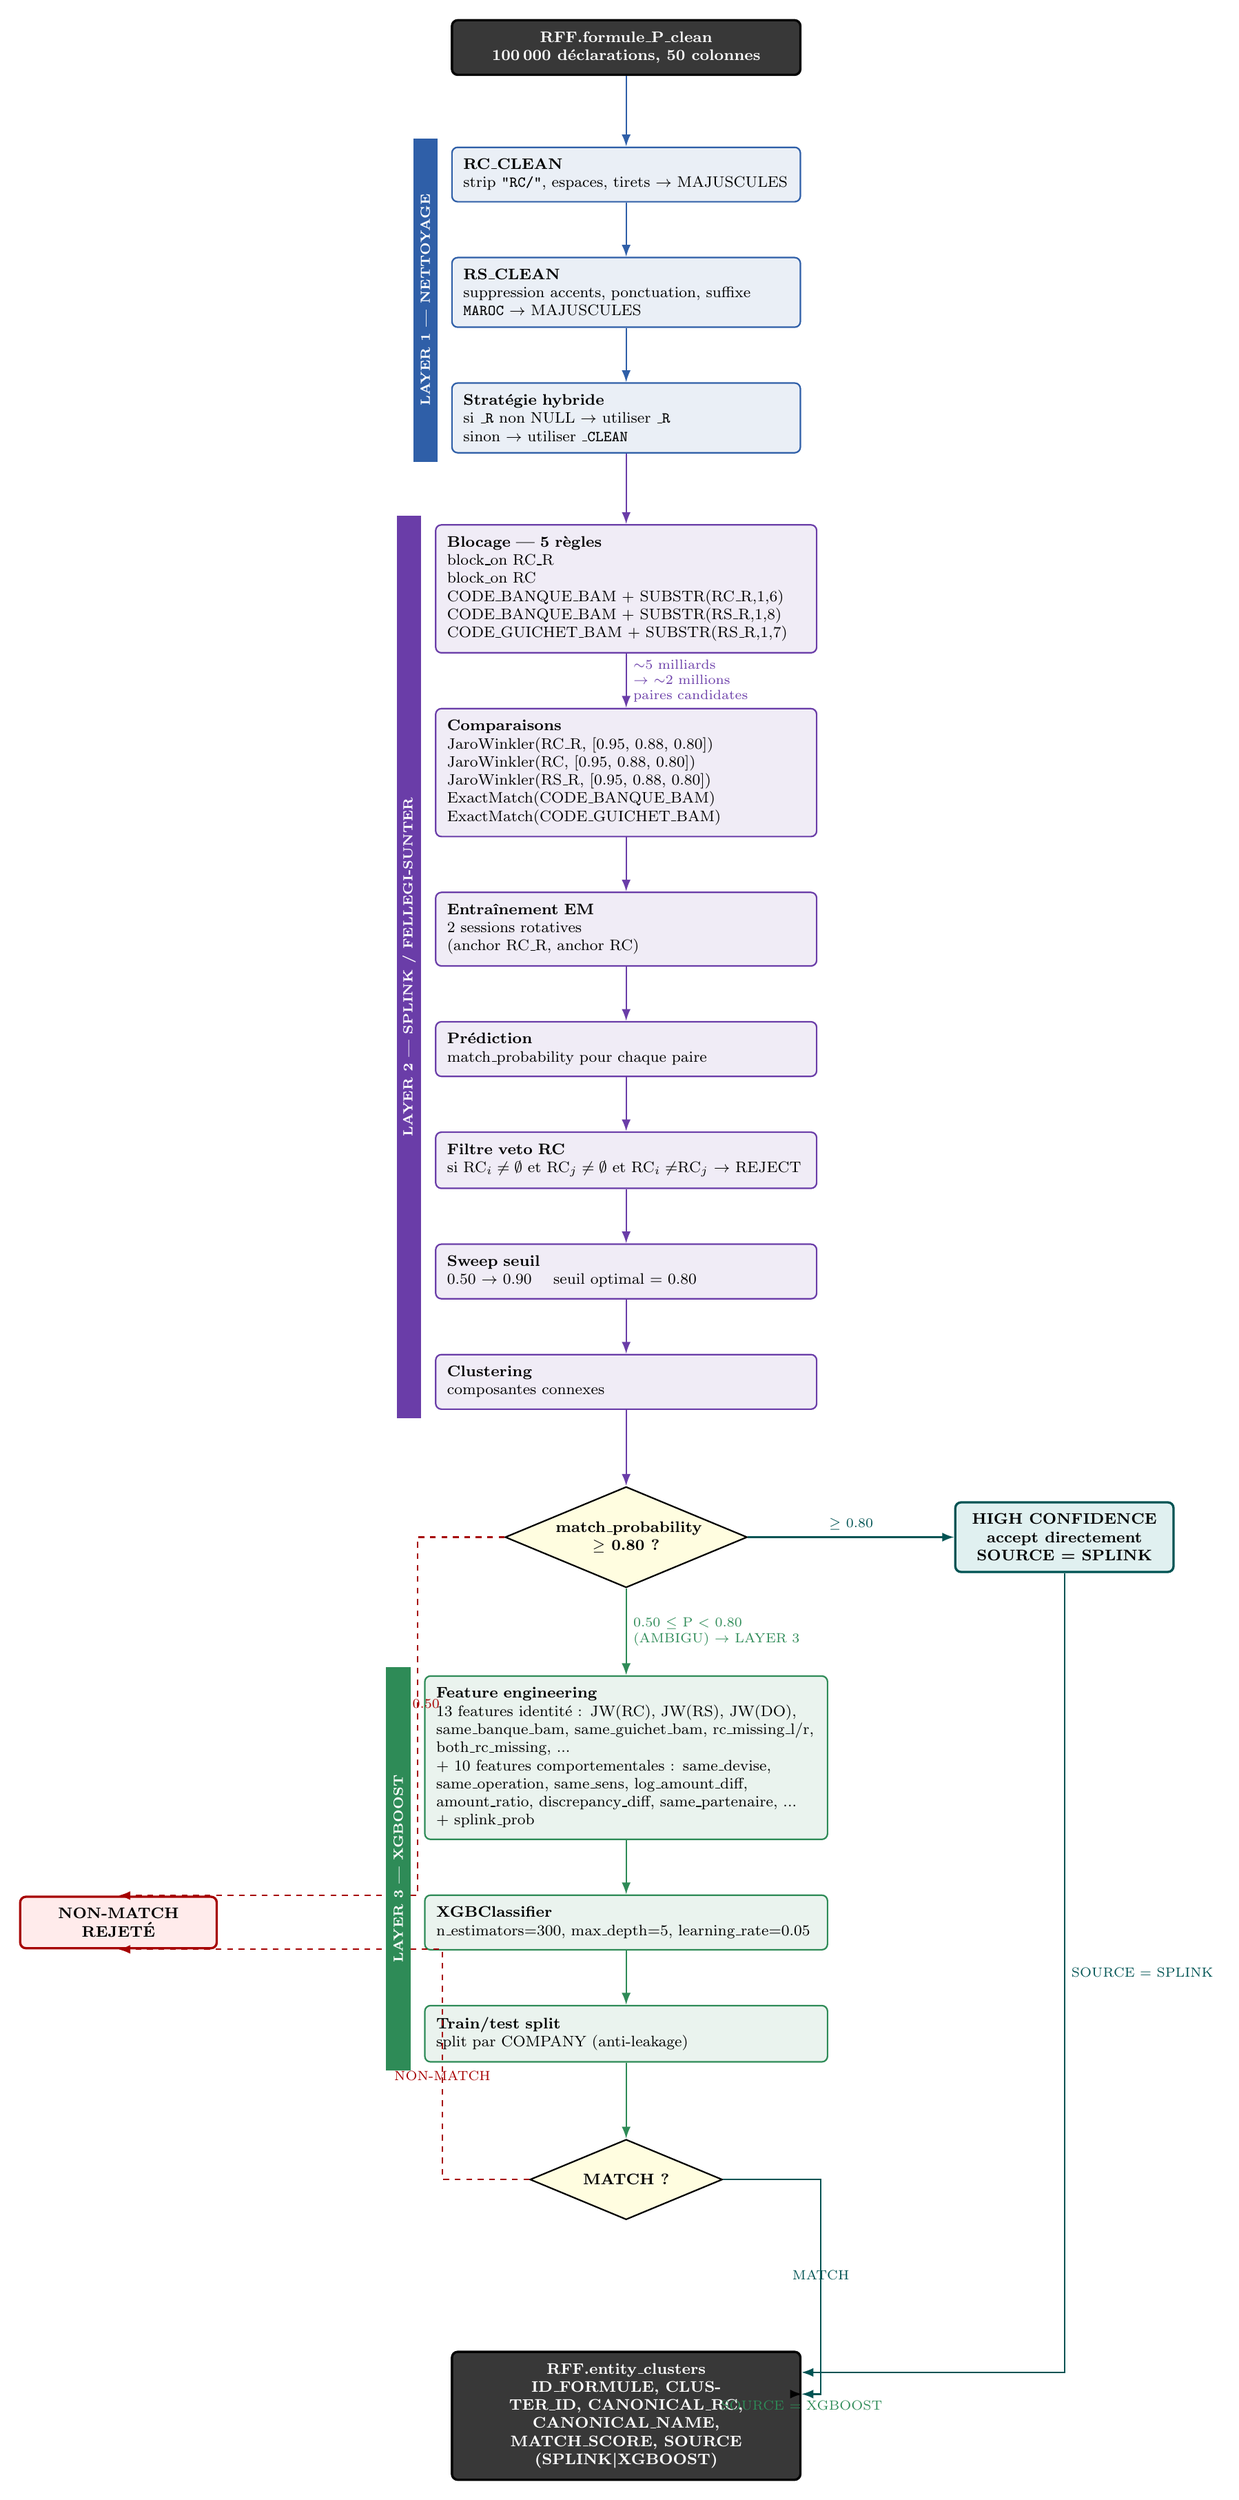
\begin{tikzpicture}[node distance=1.0cm]

% ---------------- INPUT ----------------
\node[io] (n-input) {RFF.formule\_P\_clean\\100\,000 déclarations, 50 colonnes};

% ---------------- LAYER 1 : NETTOYAGE ----------------
\node[layer1, below=1.3cm of n-input] (n-rc)
  {\textbf{RC\_CLEAN}\\strip \texttt{"RC/"}, espaces, tirets $\rightarrow$ MAJUSCULES};
\node[layer1, below=of n-rc] (n-rs)
  {\textbf{RS\_CLEAN}\\suppression accents, ponctuation, suffixe \texttt{MAROC} $\rightarrow$ MAJUSCULES};
\node[layer1, below=of n-rs] (n-hyb)
  {\textbf{Stratégie hybride}\\si \texttt{\_R} non NULL $\rightarrow$ utiliser \texttt{\_R}\\sinon $\rightarrow$ utiliser \texttt{\_CLEAN}};

% ---------------- LAYER 2 : SPLINK / FELLEGI-SUNTER ----------------
\node[layer2, below=1.3cm of n-hyb] (n-bloc)
  {\textbf{Blocage --- 5 règles}\\
   block\_on RC\_R\\
   block\_on RC\\
   CODE\_BANQUE\_BAM + SUBSTR(RC\_R,1,6)\\
   CODE\_BANQUE\_BAM + SUBSTR(RS\_R,1,8)\\
   CODE\_GUICHET\_BAM + SUBSTR(RS\_R,1,7)};
\node[layer2, below=of n-bloc] (n-comp)
  {\textbf{Comparaisons}\\
   JaroWinkler(RC\_R, [0.95, 0.88, 0.80])\\
   JaroWinkler(RC, [0.95, 0.88, 0.80])\\
   JaroWinkler(RS\_R, [0.95, 0.88, 0.80])\\
   ExactMatch(CODE\_BANQUE\_BAM)\\
   ExactMatch(CODE\_GUICHET\_BAM)};
\node[layer2, below=of n-comp] (n-em)
  {\textbf{Entraînement EM}\\2 sessions rotatives\\(anchor RC\_R, anchor RC)};
\node[layer2, below=of n-em] (n-pred)
  {\textbf{Prédiction}\\match\_probability pour chaque paire};
\node[layer2, below=of n-pred] (n-veto)
  {\textbf{Filtre veto RC}\\si RC$_i\neq\emptyset$ et RC$_j\neq\emptyset$ et RC$_i\neq$RC$_j$ $\rightarrow$ REJECT};
\node[layer2, below=of n-veto] (n-sweep)
  {\textbf{Sweep seuil}\\0.50 $\rightarrow$ 0.90 \quad seuil optimal = 0.80};
\node[layer2, below=of n-sweep] (n-clust)
  {\textbf{Clustering}\\composantes connexes};

% ---------------- DECISION 1 ----------------
\node[decision, below=1.4cm of n-clust] (n-dec1)
  {match\_probability $\geq$ 0.80 ?};

% ---------------- HIGH CONFIDENCE branch ----------------
\node[accept, right=3.8cm of n-dec1] (n-high)
  {HIGH CONFIDENCE\\accept directement\\SOURCE = SPLINK};

% ---------------- LAYER 3 : XGBOOST (ambiguous branch) ----------------
\node[layer3, below=1.6cm of n-dec1] (n-feat)
  {\textbf{Feature engineering}\\
   13 features identité : JW(RC), JW(RS), JW(DO), same\_banque\_bam,
   same\_guichet\_bam, rc\_missing\_l/r, both\_rc\_missing, ...\\
   + 10 features comportementales : same\_devise, same\_operation,
   same\_sens, log\_amount\_diff, amount\_ratio, discrepancy\_diff,
   same\_partenaire, ...\\
   + splink\_prob};
\node[layer3, below=of n-feat] (n-xgb)
  {\textbf{XGBClassifier}\\n\_estimators=300, max\_depth=5, learning\_rate=0.05};
\node[layer3, below=of n-xgb] (n-split)
  {\textbf{Train/test split}\\split par COMPANY (anti-leakage)};

% ---------------- REJECT sink (centred between the two decisions) ----------------
\node[reject, left=3.8cm of n-xgb] (n-reject) {NON-MATCH\\REJETÉ};

% ---------------- DECISION 2 ----------------
\node[decision, below=1.4cm of n-split] (n-dec2) {MATCH ?};

% ---------------- OUTPUT ----------------
\node[io, below=2.4cm of n-dec2] (n-output)
  {RFF.entity\_clusters\\ID\_FORMULE, CLUSTER\_ID, CANONICAL\_RC,\\
   CANONICAL\_NAME, MATCH\_SCORE, SOURCE (SPLINK\textbar XGBOOST)};

% ================= MAIN SPINE ARROWS =================
\draw[arr1] (n-input) -- (n-rc);
\draw[arr1] (n-rc)    -- (n-rs);
\draw[arr1] (n-rs)    -- (n-hyb);
\draw[arr2] (n-hyb)   -- (n-bloc);
\draw[arr2] (n-bloc)  -- (n-comp)
  node[midway, right, font=\scriptsize, l2violet, align=left]
  {$\sim$5 milliards\\$\rightarrow$ $\sim$2 millions\\paires candidates};
\draw[arr2] (n-comp)  -- (n-em);
\draw[arr2] (n-em)    -- (n-pred);
\draw[arr2] (n-pred)  -- (n-veto);
\draw[arr2] (n-veto)  -- (n-sweep);
\draw[arr2] (n-sweep) -- (n-clust);
\draw[arr2] (n-clust) -- (n-dec1);

% ---- decision 1 branches ----
\draw[arracc] (n-dec1.east) -- (n-high.west) node[midway, above, font=\scriptsize] {$\geq$ 0.80};
\draw[arr3]   (n-dec1.south) -- (n-feat.north)
  node[midway, right, font=\scriptsize, align=left] {0.50 $\le$ P $<$ 0.80\\(AMBIGU) $\rightarrow$ LAYER 3};
\draw[arrrej] (n-dec1.west) -- ++(-1.6,0) |- (n-reject.north)
  node[near start, above, font=\scriptsize] {$<$ 0.50};

% ---- layer 3 internal ----
\draw[arr3] (n-feat)  -- (n-xgb);
\draw[arr3] (n-xgb)   -- (n-split);
\draw[arr3] (n-split) -- (n-dec2);

% ---- decision 2 branches ----
\draw[arrrej] (n-dec2.west) -- ++(-1.6,0) |- (n-reject.south)
  node[near start, below, font=\scriptsize] {NON-MATCH};
\draw[arracc] (n-dec2.east) -- ++(1.8,0) |- ($(n-output.east)+(0,0.4)$)
  node[near start, above, font=\scriptsize] {MATCH};

% ---- merges into OUTPUT ----
\draw[arracc] (n-high.south) |- ($(n-output.east)+(0,0.8)$)
  node[near start, right, font=\scriptsize] {SOURCE = SPLINK};
\draw[arrdark] ($(n-output.east)+(0,0.4)$) -- ($(n-output.east)+(0.01,0.4)$)
  node[near start, below, font=\scriptsize, l3green] {SOURCE = XGBOOST};

% ================= LAYER SIDEBARS =================
\fill[l1blue] ($(n-rc.north west)+(-0.7,0.15)$) rectangle ($(n-hyb.south west)+(-0.25,-0.15)$);
\node[rotate=90, text=white, font=\bfseries\scriptsize] at
  ($(n-rc.north west)!0.5!(n-hyb.south west)+(-0.475,0)$) {LAYER 1 --- NETTOYAGE};

\fill[l2violet] ($(n-bloc.north west)+(-0.7,0.15)$) rectangle ($(n-clust.south west)+(-0.25,-0.15)$);
\node[rotate=90, text=white, font=\bfseries\scriptsize] at
  ($(n-bloc.north west)!0.5!(n-clust.south west)+(-0.475,0)$) {LAYER 2 --- SPLINK / FELLEGI-SUNTER};

\fill[l3green] ($(n-feat.north west)+(-0.7,0.15)$) rectangle ($(n-split.south west)+(-0.25,-0.15)$);
\node[rotate=90, text=white, font=\bfseries\scriptsize] at
  ($(n-feat.north west)!0.5!(n-split.south west)+(-0.475,0)$) {LAYER 3 --- XGBOOST};

\end{tikzpicture}
\caption{Pipeline de résolution d'entités (Entity Resolution) à 3 couches --- Office des Changes.}
\label{fig:er-pipeline}
\end{figure}
\end{landscape}
\end{document}
